\documentclass[]{article}
\usepackage[T1]{fontenc}
\usepackage{lmodern}
\usepackage{amssymb,amsmath}
\usepackage{ifxetex,ifluatex}
\usepackage{fixltx2e} % provides \textsubscript
% Set line spacing
% use upquote if available, for straight quotes in verbatim environments
\IfFileExists{upquote.sty}{\usepackage{upquote}}{}
\ifnum 0\ifxetex 1\fi\ifluatex 1\fi=0 % if pdftex
  \usepackage[utf8]{inputenc}
\else % if luatex or xelatex
  \ifxetex
    \usepackage{mathspec}
    \usepackage{xltxtra,xunicode}
  \else
    \usepackage{fontspec}
  \fi
  \defaultfontfeatures{Mapping=tex-text,Scale=MatchLowercase}
  \newcommand{\euro}{€}
\fi
% use microtype if available
\IfFileExists{microtype.sty}{\usepackage{microtype}}{}
\usepackage[margin=1in]{geometry}
\usepackage{color}
\usepackage{fancyvrb}
\newcommand{\VerbBar}{|}
\newcommand{\VERB}{\Verb[commandchars=\\\{\}]}
\DefineVerbatimEnvironment{Highlighting}{Verbatim}{commandchars=\\\{\}}
% Add ',fontsize=\small' for more characters per line
\usepackage{framed}
\definecolor{shadecolor}{RGB}{248,248,248}
\newenvironment{Shaded}{\begin{snugshade}}{\end{snugshade}}
\newcommand{\KeywordTok}[1]{\textcolor[rgb]{0.13,0.29,0.53}{\textbf{{#1}}}}
\newcommand{\DataTypeTok}[1]{\textcolor[rgb]{0.13,0.29,0.53}{{#1}}}
\newcommand{\DecValTok}[1]{\textcolor[rgb]{0.00,0.00,0.81}{{#1}}}
\newcommand{\BaseNTok}[1]{\textcolor[rgb]{0.00,0.00,0.81}{{#1}}}
\newcommand{\FloatTok}[1]{\textcolor[rgb]{0.00,0.00,0.81}{{#1}}}
\newcommand{\CharTok}[1]{\textcolor[rgb]{0.31,0.60,0.02}{{#1}}}
\newcommand{\StringTok}[1]{\textcolor[rgb]{0.31,0.60,0.02}{{#1}}}
\newcommand{\CommentTok}[1]{\textcolor[rgb]{0.56,0.35,0.01}{\textit{{#1}}}}
\newcommand{\OtherTok}[1]{\textcolor[rgb]{0.56,0.35,0.01}{{#1}}}
\newcommand{\AlertTok}[1]{\textcolor[rgb]{0.94,0.16,0.16}{{#1}}}
\newcommand{\FunctionTok}[1]{\textcolor[rgb]{0.00,0.00,0.00}{{#1}}}
\newcommand{\RegionMarkerTok}[1]{{#1}}
\newcommand{\ErrorTok}[1]{\textbf{{#1}}}
\newcommand{\NormalTok}[1]{{#1}}
\usepackage{graphicx}
% Redefine \includegraphics so that, unless explicit options are
% given, the image width will not exceed the width of the page.
% Images get their normal width if they fit onto the page, but
% are scaled down if they would overflow the margins.
\makeatletter
\def\ScaleIfNeeded{%
  \ifdim\Gin@nat@width>\linewidth
    \linewidth
  \else
    \Gin@nat@width
  \fi
}
\makeatother
\let\Oldincludegraphics\includegraphics
{%
 \catcode`\@=11\relax%
 \gdef\includegraphics{\@ifnextchar[{\Oldincludegraphics}{\Oldincludegraphics[width=\ScaleIfNeeded]}}%
}%
\ifxetex
  \usepackage[setpagesize=false, % page size defined by xetex
              unicode=false, % unicode breaks when used with xetex
              xetex]{hyperref}
\else
  \usepackage[unicode=true]{hyperref}
\fi
\hypersetup{breaklinks=true,
            bookmarks=true,
            pdfauthor={barb dornseif - saoirsegirl},
            pdftitle={An Exploration of Tooth Growth Data},
            colorlinks=true,
            citecolor=blue,
            urlcolor=blue,
            linkcolor=magenta,
            pdfborder={0 0 0}}
\urlstyle{same}  % don't use monospace font for urls
\setlength{\parindent}{0pt}
\setlength{\parskip}{6pt plus 2pt minus 1pt}
\setlength{\emergencystretch}{3em}  % prevent overfull lines
\setcounter{secnumdepth}{5}

%%% Change title format to be more compact
\usepackage{titling}
\setlength{\droptitle}{-2em}
  \title{An Exploration of Tooth Growth Data}
  \pretitle{\vspace{\droptitle}\centering\huge}
  \posttitle{\par}
  \author{barb dornseif - saoirsegirl}
  \preauthor{\centering\large\emph}
  \postauthor{\par}
  \predate{\centering\large\emph}
  \postdate{\par}
  \date{February, 2015}




\begin{document}

\maketitle


\section{Loading and Summarization of Data Set:
ToothGrowth}\label{loading-and-summarization-of-data-set-toothgrowth}

Let's load our data and look at a summary and the structure of is
contents.

\begin{Shaded}
\begin{Highlighting}[]
\KeywordTok{data}\NormalTok{(ToothGrowth); }\KeywordTok{str}\NormalTok{(ToothGrowth); }\KeywordTok{summary}\NormalTok{(ToothGrowth)}
\end{Highlighting}
\end{Shaded}

\begin{verbatim}
## 'data.frame':    60 obs. of  3 variables:
##  $ len : num  4.2 11.5 7.3 5.8 6.4 10 11.2 11.2 5.2 7 ...
##  $ supp: Factor w/ 2 levels "OJ","VC": 2 2 2 2 2 2 2 2 2 2 ...
##  $ dose: num  0.5 0.5 0.5 0.5 0.5 0.5 0.5 0.5 0.5 0.5 ...
\end{verbatim}

\begin{verbatim}
##       len        supp         dose      
##  Min.   : 4.20   OJ:30   Min.   :0.500  
##  1st Qu.:13.07   VC:30   1st Qu.:0.500  
##  Median :19.25           Median :1.000  
##  Mean   :18.81           Mean   :1.167  
##  3rd Qu.:25.27           3rd Qu.:2.000  
##  Max.   :33.90           Max.   :2.000
\end{verbatim}

We can see there are 60 observations of 3 columns, that the first and
third columns are numerics - and the second column is a factor with two
levels. The summary further tells us the quantile breakdown of each of
the numeric columns. If we lookup the short documentation on the dataset
\href{https://stat.ethz.ch/R-manual/R-devel/library/datasets/html/ToothGrowth.html}{link}
we see the following description ``The response is the length of
odontoblasts (teeth) in each of 10 guinea pigs at each of three dose
levels of Vitamin C (0.5, 1, and 2 mg) with each of two delivery methods
(orange juice or ascorbic acid).''

So we know that we have a growth in the length of of teeth for six(6)
groupings of 10 guinea pigs where each group is given one of three(3)
dosage amounts via one or the other of two(2) delivery methods (column =
``supp''). Let's take a look at how length groups by dose and delivery
separately.

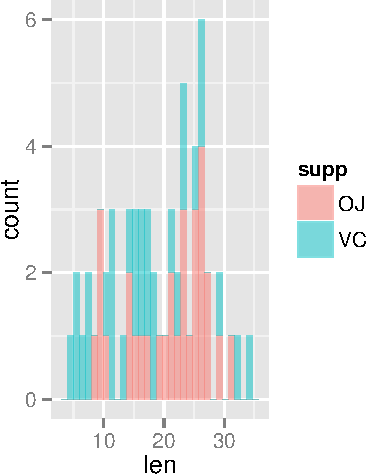
\includegraphics{06_Project1b_files/figure-latex/plotting1-1.pdf}
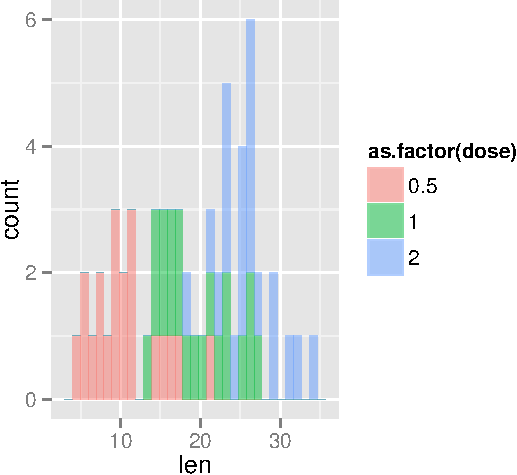
\includegraphics{06_Project1b_files/figure-latex/plotting2-1.pdf}

We can see by the clustering by color, that there are distinct
distributions of lengths by dose (when used as a factor variable) and
less so by delivery. And although we see there is some overlap between
each grouping, it is pretty safe to say that the greater the dose, the
greater the efficacy. Our first hypothesis is that the overlaps may
suggest that we are not sure how or if the delivery method impacts this
simple observation. So we will test each dosage against the two delivery
methods using a standard t-Test to detirmine if the variability is
intrinsic to the dosage level, or is impacted by the delivery method.

Because we see that the spread of each density is different as well, we
will need to assume that the variance for each group varies, even though
the number of observations in each sample is the same; this will impact
the results generated by the t-Test.

\section{Using Means and Confidence Intervals to Compare Growth by
Delivery and
Dosage.}\label{using-means-and-confidence-intervals-to-compare-growth-by-delivery-and-dosage.}

So let's start by isolating the dosage (2.0 mg) that appears to give the
best growth results, and see if the delivery method shows any
distinction in efficacy. The groups are sorted alphabetically, so OJ
will take the position of having the larger mean with which to test VC
against. Let's see if this is true for a dosage of 2.0 mg.

\begin{table}[ht]
\centering
\begin{tabular}{rrr}
  \hline
 & OJ = Orange Juice & VC = Asorbic Acid \\ 
  \hline
Means of each Group & 26.06 & 26.14 \\ 
  Confidence of the Difference & -3.80 & 3.64 \\ 
   \hline
\end{tabular}
\caption{Means and Confidence Intervals for Dosage 2.0 mg} 
\end{table}

Using the t-test to derive the Means of two groups of equal size, and
the Confidence Interval of the difference between those Means when both
receive the same dosage of 2.0 mg. we see that there is little
distinction between Mean tooth length when receiving orange juice (OJ)
versus Asorbic Acid (VC) as the method of delivery. Further, the
Confidence Interval clearly straddles zero, so we must conclude that at
this dosage, method of delivery is not a relavant factor the growth
outcome.

But given the observed histograms we cannot conclude that this holds
true for all dosages. So let's try the 0.5 mg dosage, which shows the
tightest clustering in the histogram.

\begin{table}[ht]
\centering
\begin{tabular}{rrr}
  \hline
 & OJ = Orange Juice & VC = Asorbic Acid \\ 
  \hline
Means of each Group & 13.23 & 7.98 \\ 
  Confidence of the Difference & 1.72 & 8.78 \\ 
   \hline
\end{tabular}
\caption{Means and Confidence Intervals for Dosage 0.5 mg} 
\end{table}

Here we see the different relationship. Althought the Mean itself is
significantly lower than at the higher dosage, using OJ provides a
significantly higher mean growth result (by 5.25) and the confidence
interval is significantly above zero. Here, we can conclude that
delivery method does impact efficacy and that orange juice is the
preferred method.

Given such divergent outcomes, let's try our third dosage (1.0 mg) and
see which camp it most resembles.

\begin{table}[ht]
\centering
\begin{tabular}{rrr}
  \hline
 & OJ = Orange Juice & VC = Asorbic Acid \\ 
  \hline
Means of each Group & 22.70 & 16.77 \\ 
  Confidence of the Difference & 2.80 & 9.06 \\ 
   \hline
\end{tabular}
\caption{Means and Confidence Intervals for Dosage 1.0 mg} 
\end{table}

Interestingly, the 1.0 mg dosage not only appears to provide a better
mean efficacy than the 0.5 mg dosage it also shows a greater distiction
in efficacy between the two delivery methods with OJ providing higher
measured growth by 5.93 and with a narrower Confidence Interval that the
actual difference in the population Means will consistently bear this
out. However the amount of growth for OJ delivered Vitamin C does not
exceed either delivery method of the 2.0 dosage. So we are left with a
conondrum given we have no data on the doage 1.5 mg which lies between
these two groups.

\section{Conclusions}\label{conclusions}

Not knowing the cost of each of the dosages by delivery method, the
impacts of 1.5 mg dosing nor the potential negative impacts of
overdosing on the test subjects, it would appear that using orange juice
at the dosage of 1.0 mg is the most reliable method and dosage to
acheive the greatest potential impact on tooth growth for the least
amount of intervention/cost.

\section{Appendix - Code Chunks Using echo =
FALSE}\label{appendix---code-chunks-using-echo-false}

Echo=TRUE is replaced with eval=TRUE

\begin{Shaded}
\begin{Highlighting}[]
\KeywordTok{library}\NormalTok{(ggplot2)}
\KeywordTok{ggplot}\NormalTok{(ToothGrowth, }\KeywordTok{aes}\NormalTok{(len, }\DataTypeTok{fill =} \NormalTok{supp)) +}\StringTok{ }\KeywordTok{geom_histogram}\NormalTok{(}\DataTypeTok{alpha =} \FloatTok{0.5}\NormalTok{)}

\KeywordTok{ggplot}\NormalTok{(ToothGrowth, }\KeywordTok{aes}\NormalTok{(len, }\DataTypeTok{fill =} \KeywordTok{as.factor}\NormalTok{(dose))) +}\StringTok{ }\KeywordTok{geom_histogram}\NormalTok{(}\DataTypeTok{alpha =} \FloatTok{0.5}\NormalTok{)}
\end{Highlighting}
\end{Shaded}

Manipulations of ToothGrowth data - repeated three times; once for each
dosage grouping.

\begin{Shaded}
\begin{Highlighting}[]
\NormalTok{TGs2 <-}\StringTok{ }\KeywordTok{subset}\NormalTok{(ToothGrowth, dose %in%}\StringTok{ }\DecValTok{2}\NormalTok{)}
\NormalTok{TGs2 <-}\StringTok{ }\KeywordTok{t.test}\NormalTok{(len~supp, }\DataTypeTok{paired =} \OtherTok{FALSE}\NormalTok{, }\DataTypeTok{var.equal=}\OtherTok{FALSE}\NormalTok{, }\DataTypeTok{data=}\NormalTok{TGs2) }\CommentTok{# grab the output of the function}
\NormalTok{TGs2c <-}\StringTok{ }\KeywordTok{c}\NormalTok{(}\KeywordTok{as.vector}\NormalTok{(TGs2$conf[}\DecValTok{1}\NormalTok{]), }\KeywordTok{as.vector}\NormalTok{(TGs2$conf[}\DecValTok{2}\NormalTok{]))}
\NormalTok{TGs2m <-}\StringTok{ }\KeywordTok{c}\NormalTok{(}\KeywordTok{as.vector}\NormalTok{(TGs2$estimate[}\DecValTok{1}\NormalTok{]), }\KeywordTok{as.vector}\NormalTok{(TGs2$estimate[}\DecValTok{2}\NormalTok{]))}
\end{Highlighting}
\end{Shaded}

\begin{Shaded}
\begin{Highlighting}[]
\KeywordTok{library}\NormalTok{(xtable)}
\NormalTok{table1 <-}\StringTok{ }\KeywordTok{rbind}\NormalTok{( TGs2m, TGs2c)}
\KeywordTok{rownames}\NormalTok{(table1) <-}\StringTok{ }\KeywordTok{c}\NormalTok{(}\StringTok{"Means of each Group"}\NormalTok{, }\StringTok{"Confidence of the Difference"}\NormalTok{)}
\KeywordTok{colnames}\NormalTok{(table1) <-}\StringTok{ }\KeywordTok{c}\NormalTok{(}\StringTok{"OJ = Orange Juice"}\NormalTok{, }\StringTok{"VC = Asorbic Acid"}\NormalTok{)}
\KeywordTok{print}\NormalTok{(}\KeywordTok{xtable}\NormalTok{(table1, }\DataTypeTok{format =} \StringTok{"markdown"}\NormalTok{, }\DataTypeTok{caption =} \StringTok{"Means and Confidence Intervals for Dosage 2.0 mg"}\NormalTok{),}\DataTypeTok{comment=}\OtherTok{FALSE}\NormalTok{)}
\end{Highlighting}
\end{Shaded}

\end{document}
